\chapter{Delft3D Model}
\label{chap:Delft3DModel}
This chapter presents the setup and application of the Delft3D model developed to understand the flow behaviour in the study area, with a focus on the confluence area were sand extraction occurs. In addition, the model results are used to identify locations along the river that are prone to erosion. The model was set up as a two-dimensional, depth-averaged model in which sediment transport and morphological changes are not considered. The time period simulated is 25 and 26 September 2025, the two days at which field measurements were taken. The field measurements from these days are used for boundary conditions and calibration of the model.

\section{Model approach}
In this section, the Delft3D model setup used to simulate the hydrodynamic response of the system is explained. The setup of the model involves defining the computational grid, processing the bathymetry, specifying boundary and initial conditions and finally selecting appropriate physical and numerical parameters.

Since no existing grid was available for the area of interest, the grid was generated using the RGFGRID tool in Delft3D. As a starting point, a land boundary file similar to the one shown in Figure \ref{fig:cross section domain} was used. By drawing splines with a decreasing spacing towards the confluence, the grid resolution was refined for the region of hydrodynamic interest. This approach ensures that the model captures the flow behaviour at the confluence with high accuracy while maintaining computational efficiency in less critical areas. After generating the grid, further refinements were made to ensure that the grid contains at least 20 cells in a cross section near the confluence and around 10 cells in a cross section far away from the confluence. When generating the grid, it was made sure to limit the aspect ratio to 2.0. The generated grid is shown in Figure \ref{fig: Grid Guazu Delft3D}. The generated computational grid has 1044 grid cells in M-direction, 1043 cells in N-direction, and 91706 grid elements. The grid size at the confluence is around 20x20 meters and the grid size at the upstream boundary near Ibicuy is 75x125 meters. 

\begin{figure}[h]
    \centering
    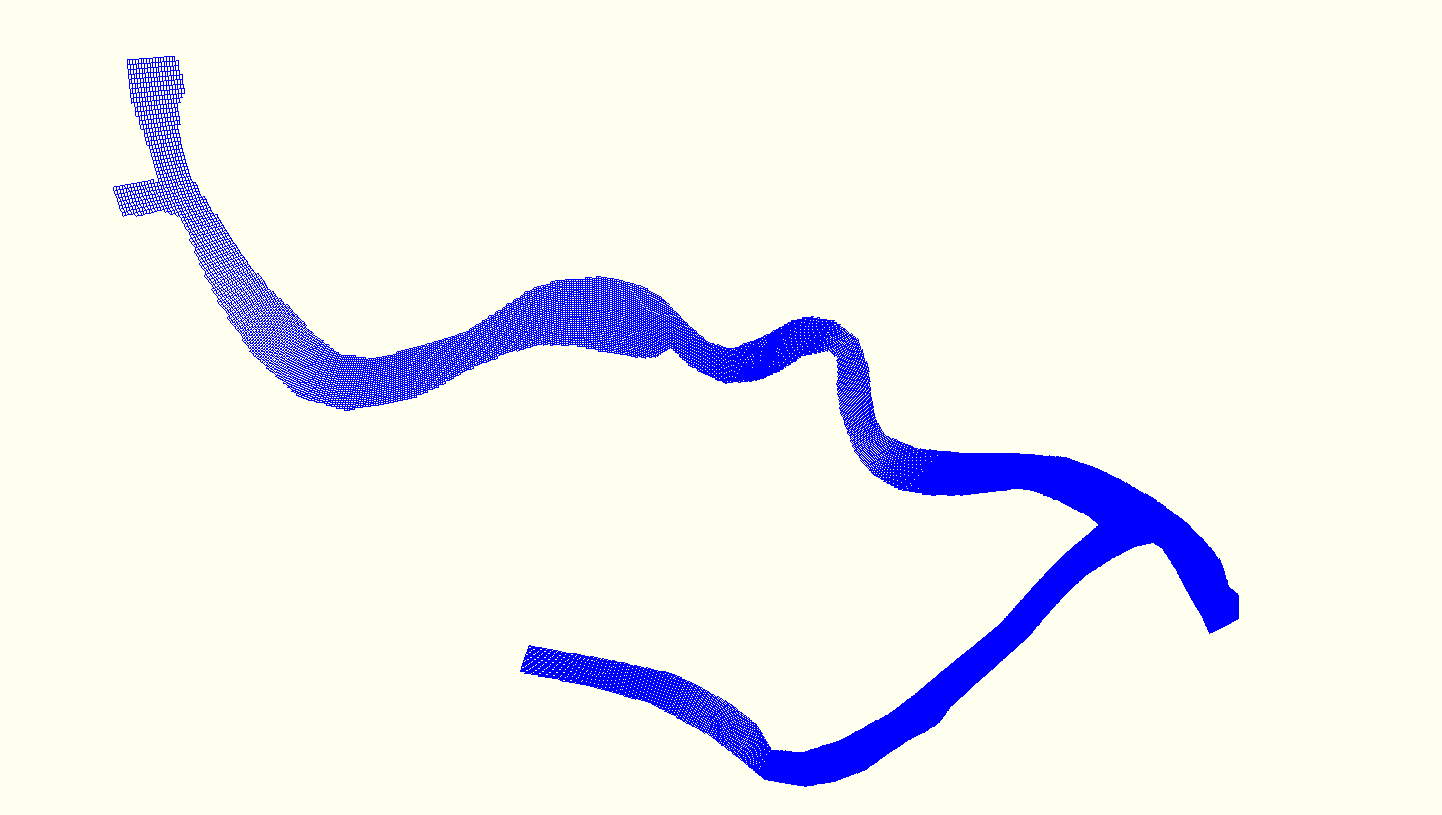
\includegraphics[width=0.75\textwidth, height=8cm]{figures/ch7/Grid_Guazu.png}
    \caption{Generated grid for the Delft3D model.}
    \label{fig:Grid_Guazu_Delft3D}
\end{figure}


The bathymetry was derived from a Digital Elevation Model (DEM) from 2019, which was provided by INA. This DEM was used to create samples containing geospatial coordinates and the corresponding depths. Using the QUICKIN tool in Delft3D, these samples were interpolated onto the computational grid. For this interpolation, Grid Cell Averaging was applied with the minimum number of averaging points set to one. Grid Cell Averaging was preferred over Triangular Interpolation as it is computationally less expensive, and more samples were available than grid points \autocite{deltaresQUICKINUserManual2025}. Lastly, Internal Diffusion was applied, with the number of internal diffusion steps set to 1000, to smooth sharp gradients and fill in missing values. The interpolated bathymetry is shown in Figure \ref{fig: Bathymetry Delft3D}. The maximum depth of 40.403 m occurs just downstream of the confluence. 

\begin{figure}[H]
    \centering
    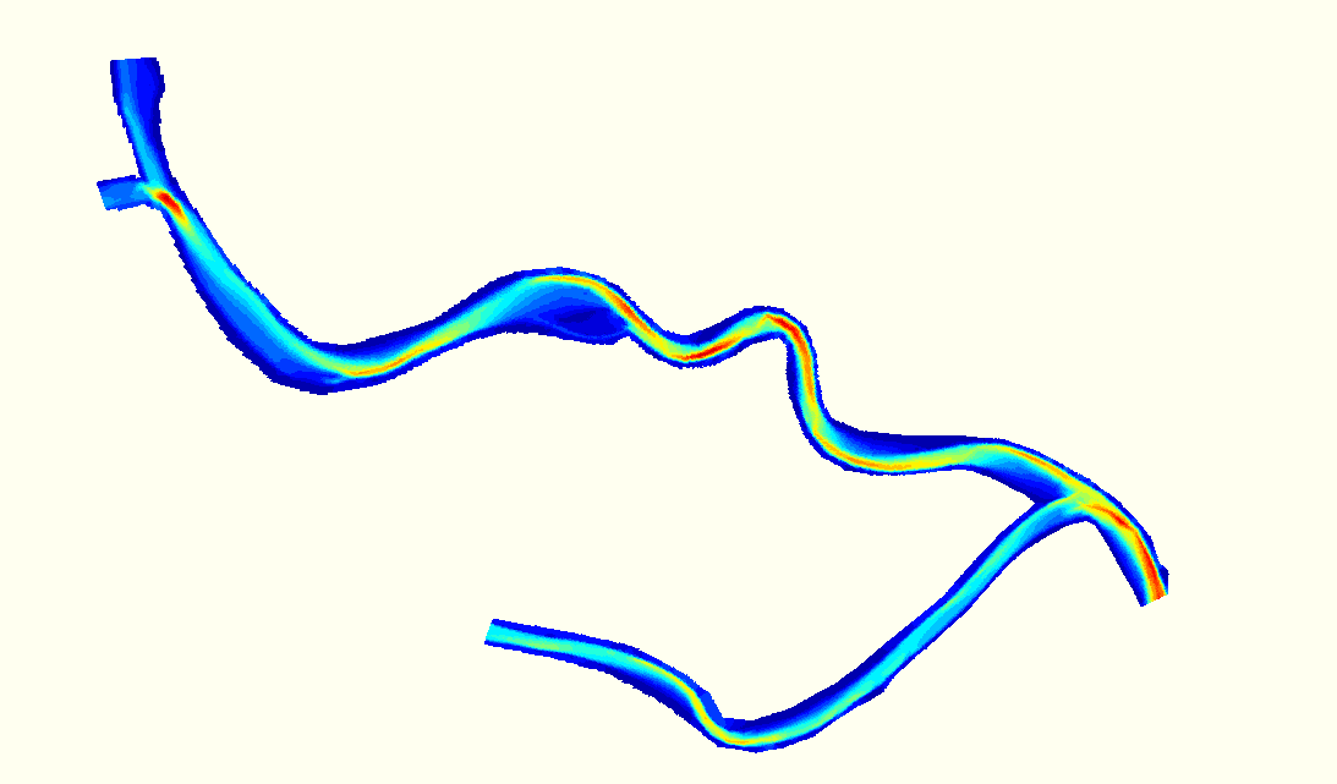
\includegraphics[width=0.75\textwidth, height=8cm]{figures/ch7/Bathymetry_Gueazu_Delft3D.png}
    \caption{Bathymetry Delft3D model.}
    \label{fig:Bathymetry_Delft3D}
\end{figure}

In order to validate the use of the 2019 DEM for creating the bathymetry, cross sections from the generated bathymetry were compared with measurements obtained by the ADCP during the field campaign. The comparison of the bathymetries of the three cross sections is shown in Figure \ref{fig:bathymetry_cross_sections}. Although the interpolated and measured bathymetries are not exactly the same, the overall shape and depths are very similar, ensuring that the Delft3D simulations accurately represent the current hydraulic conditions.

\begin{figure}[H]
    \centering
    % Top row: two subfigures side by side
    \begin{subfigure}[t]{0.48\linewidth}
        \centering
        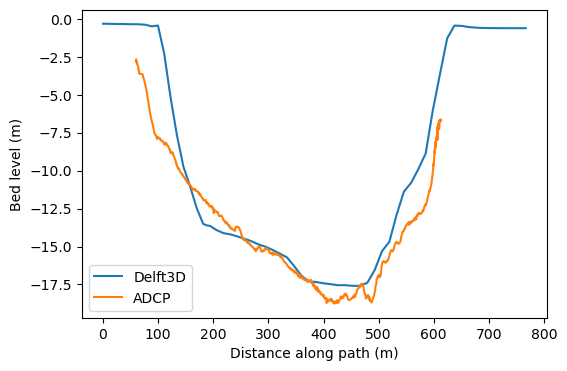
\includegraphics[width=\linewidth,height=0.7\linewidth]{figures/ch7/Bathymetry_cs1.png}
        \caption{Cross section 1}
        \label{fig:bathy_cs1}
    \end{subfigure}
    \hfill
    \begin{subfigure}[t]{0.48\linewidth}
        \centering
        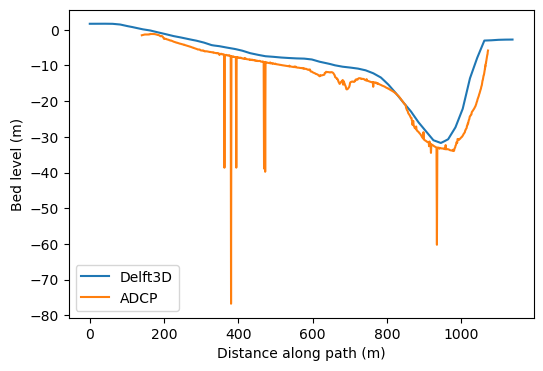
\includegraphics[width=\linewidth,height=0.7\linewidth]{figures/ch7/Bathymetry_cs2.png}
        \caption{Cross section 2}
        \label{fig:bathy_cs2}
    \end{subfigure}

    % Bottom row: one centered subfigure
    \vspace{1em}
    \begin{subfigure}[t]{0.48\linewidth}
        \centering
        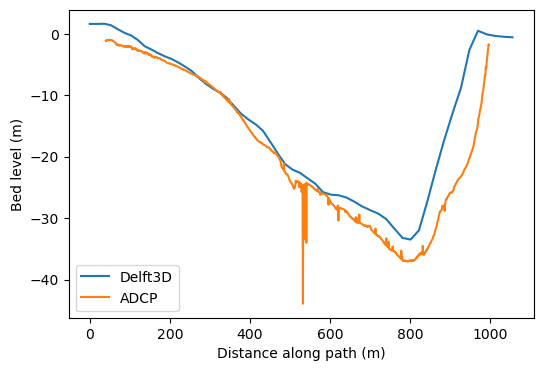
\includegraphics[width=\linewidth,height=0.7\linewidth,keepaspectratio]{figures/ch7/Bathymetry_cs3.png}
        \caption{Cross section 3}
        \label{fig:bathy_cs3}
    \end{subfigure}

    \caption{Bed levels along the three analysed cross sections: (a) Cross section 1, (b) Cross section 2, and (c) Cross section 3.}
    \label{fig:bathymetry_cross_sections}
\end{figure}

The computational grid shown in Figure~\ref{fig: Grid Guazu Delft3D} has four open boundaries where boundary conditions must be imposed. For the downstream boundary at Brazo Largo, a water level time series with measurements taken every 20 minutes was used, see Figure \ref{fig: Downstream bc}. For the other three boundaries at Río Talabera, Río Ibicuy, and Río Paraná, total discharge time series were applied. Since no discharge data were available for these locations, discharge results from a one-dimensional HEC-RAS model at Brazo Largo were provided by INA. Using the discharge measurements from the field campaign, assumptions were made of the percentage of total discharge distributed across the domain. These ratios, derived from Table~\ref{tab:discharges fieldwork}, were subsequently multiplied by the Brazo Largo discharge series to determine the appropriate boundary conditions for the remaining boundaries. The three upstream boundary conditions are shown in Figure \ref{fig: Upstream bc}.

\begin{figure}[H]
    \centering
    \begin{minipage}[t]{0.48\linewidth}
        \centering
        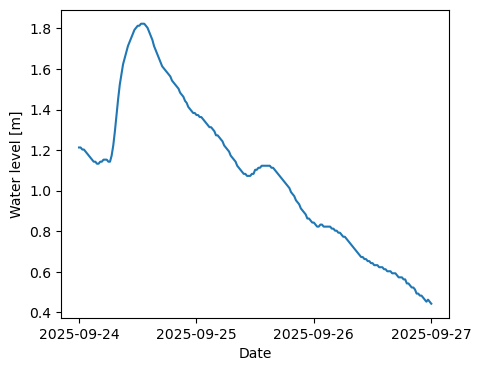
\includegraphics[height=6cm]{figures/ch7/Downstream_bc.png}
        \caption{Downstream water level boundary condition.}
        \label{fig: Downstream bc}
    \end{minipage}
    \hfill
    \begin{minipage}[t]{0.48\linewidth}
        \centering
        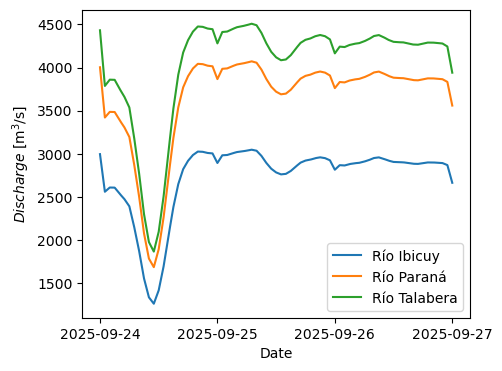
\includegraphics[height=6cm]{figures/ch7/Upstream_bc.png}
        \caption{Upstream discharge boundary conditions.}
        \label{fig: Upstream bc}
    \end{minipage}
\end{figure}

For the initial water level, the water level was used at the start of the first simulated day (1.213 m). Since the period of interest is 25 and 26 September 2025, the simulation was started on 24 September 2025 to allow for model spin-up.

\subsubsection{Physical and numerical parameters}
For the hydrodynamic simulation, a time step of 0.2 minutes was used to ensure that the Courant number remained below 1.0, thereby maintaining numerical stability while remaining computationally efficient. The bed roughness was defined using the Manning formula with a Manning's roughness coefficient ($n$) of 0.025 in both the longitudinal (U) and lateral (V) directions, which corresponds to moderately rough river beds. In order to account for the secondary flow in river bends and the confluence, a secondary flow coefficient ($\beta_c$) of 0.5 is used. This coefficient determines the fraction of shear stress taken into account in the momentum equation due to secondary flow. 

The horizontal eddy viscosity and horizontal eddy diffusivity were set to 1 m\textsuperscript{2}/s and 2 m\textsuperscript{2}/s respectively. These values were chosen to provide realistic horizontal momentum and scalar transport. Large values for the horizontal eddy viscosity and horizontal eddy diffusivity can lead to excessive numerical smoothing. The HLES turbulence model was not activated to calculate the viscosity and diffusivity in the base run, because simulations with HLES activated are computationally more expensive. HLES resolves smaller turbulent eddies explicitly, which requires a smaller time step, hence why it is computationally more expensive. Instead, the influence of the HLES turbulence model is evaluated in the sensitivity analysis.

\section{Model Calibration}
The Delft3D model was calibrated to ensure that the simulated hydrodynamic conditions accurately represent the real-life flow conditions. The calibration was done by comparing the model's water elevation near Ibicuy to a measured water elevation time series. Additionally, the simulated depth-averaged velocities in the three cross sections near the confluence are compared to the ADCP measurements from the field campaign. The calibration primarily focused on adjusting the Manning roughness coefficient, as this parameter has the highest influence on flow velocities and water depth.

In addition to the initial Manning roughness coefficient ($n$) of 0.025, the model was tested with roughness coefficients of 0.01, 0.02, and 0.05.The resulting water levels at Ibicuy are shown in Figure \ref{fig: WL calibration}. It can be clearly observed that a higher bed roughness leads to higher water elevations. Of all the values tested, a Manning coefficient of 0.02 was found to result in the most accurate water elevations.

\begin{figure}[H]
    \centering
    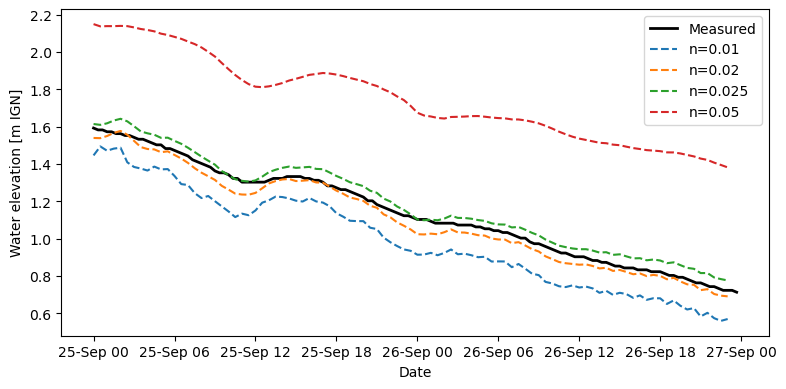
\includegraphics[width=1\linewidth]{figures/ch7/WL_calibration.png}
    \caption{Water elevations near Ibicuy for measurements (solid line) and model output (dashed line).}
    \label{fig: WL calibration}
\end{figure}

\begin{figure}[H]
    \centering
    % Top row: two subfigures side by side
    \begin{subfigure}[t]{0.48\linewidth}
        \centering
        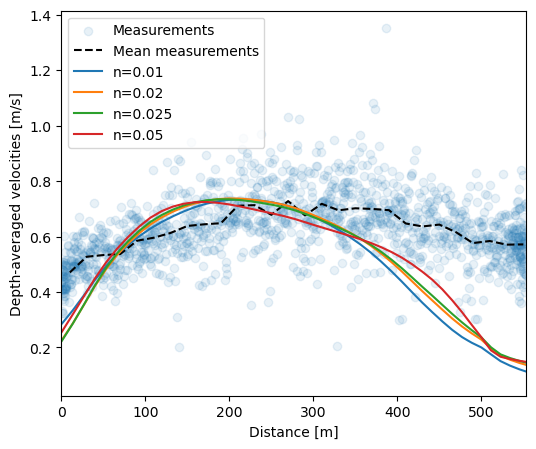
\includegraphics[width=\linewidth, height=6cm, keepaspectratio]{figures/ch7/dav_cal_1.png}
        \caption{Cross section 1}
        \label{fig: dav cal cs1}
    \end{subfigure}
    \hfill
    \begin{subfigure}[t]{0.48\linewidth}
        \centering
        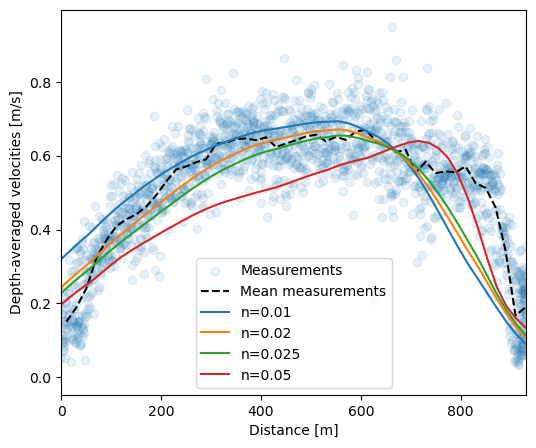
\includegraphics[width=\linewidth, height=6cm, keepaspectratio]{figures/ch7/dav_cal_2.png}
        \caption{Cross section 2}
        \label{fig: dav cal cs1}
    \end{subfigure}
    % Bottom row: one centered subfigure
    \vspace{1em}
    \begin{subfigure}[t]{0.48\linewidth}
        \centering
        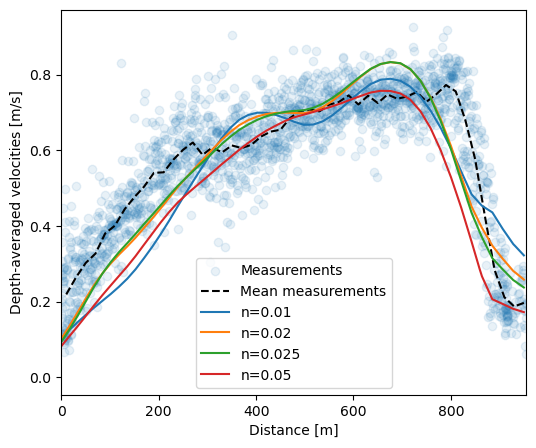
\includegraphics[width=\linewidth, height=6cm, keepaspectratio]{figures/ch7/dav_cal_3.png}
        \caption{Cross section 3}
        \label{fig: dav cal cs1}
    \end{subfigure}
    \caption{Measured and simulated depth-averaged velocities for the three cross sections.}
    \label{fig: Depth-averaged velocity calibration}
\end{figure}

Figure \ref{fig: Depth-averaged velocity calibration} shows the measured and simulated depth-averaged velocities for different Manning coefficients. In general, lower bed roughness leads to higher flow velocities. However, the effect of the bed roughness on the flow velocities is less strong than the effect on the water elevation. In addition, different values for the roughness coefficient were found to slightly affect the shape of the depth-averaged velocities profiles. From Figure \ref{fig: Depth-averaged velocity calibration} it can be seen that using a Manning coefficient of 0.02 results in realistic depth-averaged velocities for cross section 2 and 3, both located in the Paraná Guazú. While the magnitude of the flow velocities is correct for cross section 1 (located in the Río Talabera), the shape of the velocity profile does not match the measured data. This discrepancy can be explained by the use of a uniform bed roughness coefficient for the entire area of interest, which may not accurately represent the different rivers.

\section{Model results}


\begin{figure}[H]
    \centering
    \begin{minipage}[t]{0.48\linewidth}
        \centering
        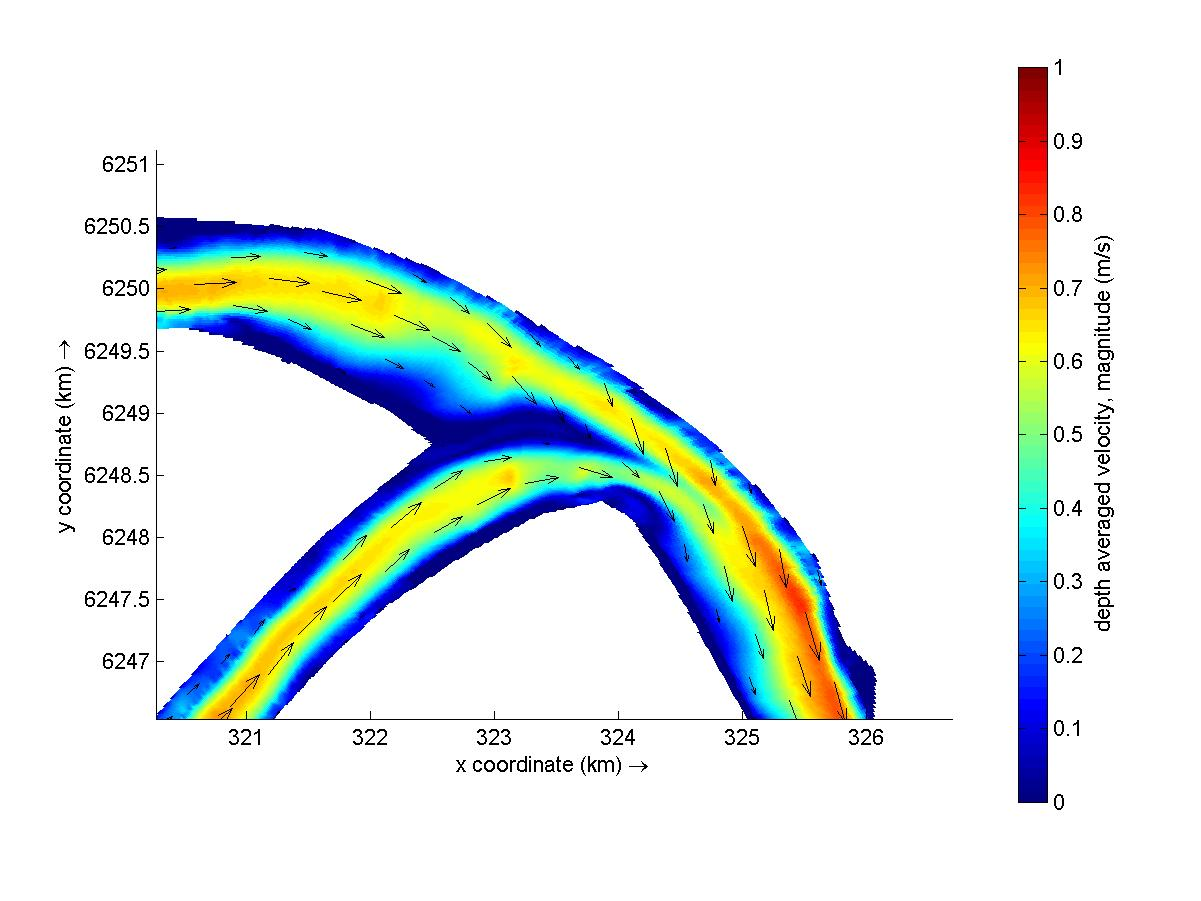
\includegraphics[height=6.5cm]{figures/ch7/dav_confluence.jpg}
        \caption{Magnitude of the depth-averaged flow velocities at the confluence.}
        \label{fig: dav confluence}
    \end{minipage}
    \hfill
    \begin{minipage}[t]{0.48\linewidth}
        \centering
        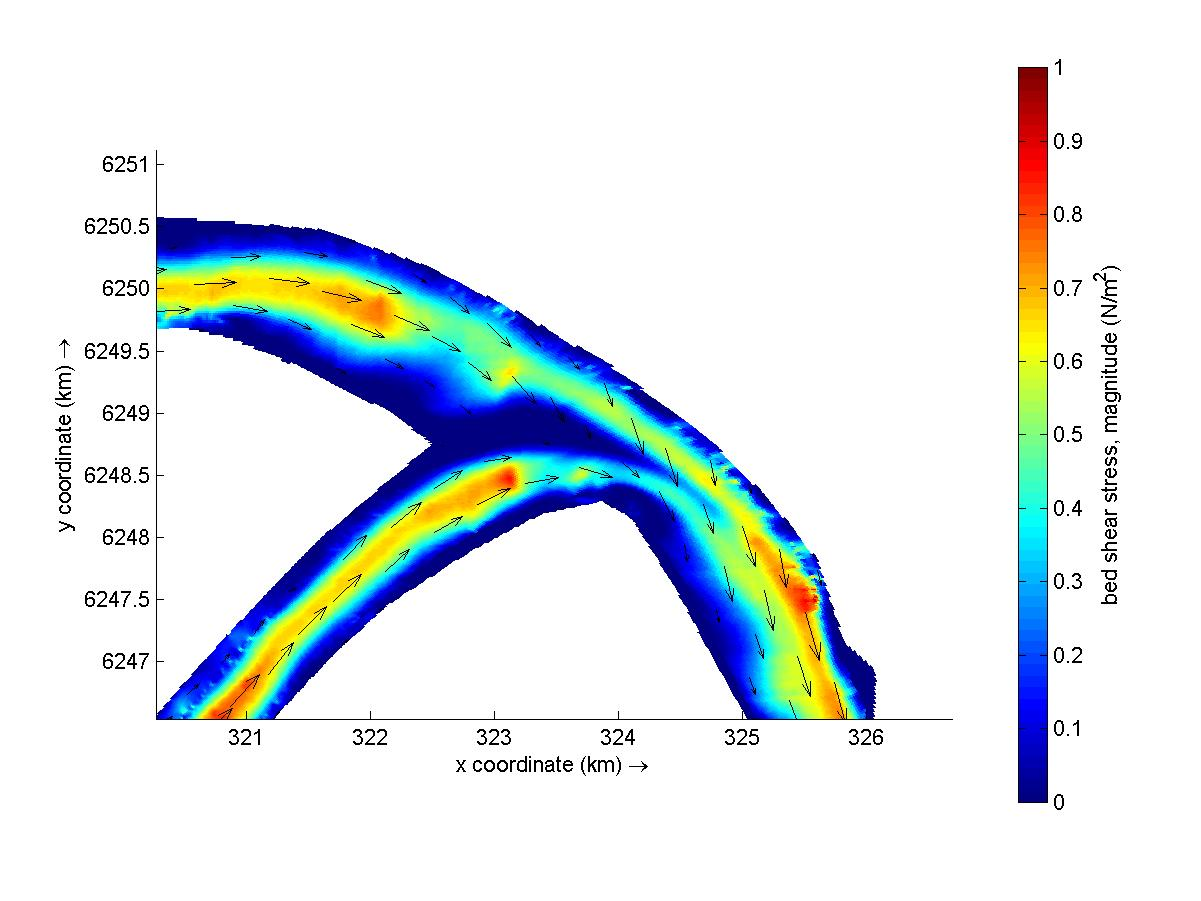
\includegraphics[height=6.5cm]{figures/ch7/Bed_shear_confluence.jpg}
        \caption{Magnitude of the bed}
        \label{fig: bed shear confluence}
    \end{minipage}
\end{figure}

\subsection{Sensitivity analysis}



